\chapter{Experimental setup}
\label{Experiment}
The \gls{LHC} successfully began circulating its first protons within its 27 km of underground tunnel on the 10th of September, 2008.  
On the 23rd of November the following year the first collisions were recorded~\cite{FirstCollisions}, signalling the beginning of the LHC's era at the forefront of the high energy frontier.  
In the years that have passed since the LHC has been consistently pushing to more frequent collisions at higher energies, allowing the experiments along its ring to explore and extend the boundaries of human knowledge.  

This chapter will describe the technology that allows these studies to be performed.  
First a walk through of the LHC acceleration complex will be provided.  
This will be followed by a description of the ATLAS detector which will be broken into the various subdetectors which make up ATLAS and the methods they use to accomplish their given tasks.   

\section{The Large Hadron Collider}
\label{Sec:LHC}

The parts of a particle accelerator can be broken down into two functional categories: rf cavities which use electric fields to accelerate particles, and magnets which are used to confine the accelerated particles.  
Circular accelerators come in two distinct flavours: cyclotrons which contain the beam using a fix strength magnetic field but allow for the radius of the circle to increase, and synchrotrons which maintain a fixed radius by increasing the magnetic field strength to compensate for the increasing energy of the accelerating particles.  
The LHC fits into the second of these categories.  

Designing to single synchrotron accelerator to accelerate bunches of protons to the energies attained at the LHC would be a difficult and expensive task.
One requirement would be the ability to finely control the field in the superconducting electromagnets used to contain the particle beam in the ring over several orders of magnitude.  
A much more cost effective approach would involve using existing machines to accomplish at least part of this task, and that's exactly the approach used at the LHC.  

The oldest component of the modern day LHC acceleration facility is the Proton Synchrotron, or PS, which was built in the 1950's which was designed to accelerate up to 10$^{10}$ protons per pulse to 26 GeV.  
The low energy at which protons were being injected into the PS was limiting the number of protons which could be injected into the ring, so in 1972 the PS booster was added.  
The PS Booster consists of four superimposed synchrotron rings which accelerated protons to 1.4 GeV before they entered the PS, allowing the PS to contain as many as 10$^{13}$ protons.  
In 1978 the linear accelerator which had been injecting protons into the PS Booster, known as the linac, was replaced by linac2, a machine which accelerates protons originating in a bottle of hydrogen gas to 50 MeV in longer pulses than its predecessor, allowing the PS Booster to be used to it's full design potential~\cite{PSHistory}~\cite{PSHistory2}.  

After the PS the protons are injected into the Super Proton Synchrotron (SPS), a machine which in 1976 when it was turned on had the ability to accelerate protons to 400 GeV, the second highest energy attainable by accelerator at that time.  
The SPS may be most well known as the machine that allowed for the discovery of both the W and Z bosons by the UA1 and UA2 collaborations.  
It may be worth noting that it takes several fills of the PS to fill the SPS, and it will again take several fills of the SPS to fully fill the LHC.  
The SPS is now the final pre-injector into the LHC, accelerating the protons up to 450 GeV before they enter the LHC itself.  

The LHC is a machines that was designed to use 16 RF cavities to accelerate 2808 bunches, each with 1.15x$10^{11}$ protons, to 7 TeV per proton.  
These bunches travel the 27 km around the ring of the LHC being held in place by 1232 8.33 Tesla superconducting dipole magnets which bend the beam, along with a number of additional magnets which help keep the beam focused~\cite{LHCTDR}.  
The LHC then crosses these counter rotating beams at four points along the beam line (the four experiments listed in~\ref{Sec:Experi}) every 25 ns, where up to 40 interactions are recorded per crossing.  

One measure of the collider's performance is it's luminosity, a description of the number of particles per unit area per unit time, which directly relates to the number of collisions per unit time and therefore the probability of obtaining a given final state per unit time.  
The LHC's design luminosity is approximately 20 times the maximum luminosity of its predecessor, the Tevatron ($10^{34}$ cm$^{-2}$s$^{-1}$ vs. 4 x $10^{32}$ cm$^{-2}$s$^{-1}$), and early in the 2016 data taking period the LHC has already started recording personal highs (8.8 x $10^{33}$ cm$^{-2}$s$^{-1})$

\section{The ATLAS Experiment}
\label{Sec:ATLAS}

\subsection{The ATLAS Coordinate System}

Before laying out the design and components of the ATLAS detector we should first establish the coordinate which will be used.  
The origin of the coordinate system that is used in ATLAS is at the geometric centre of the ATLAS detector.  
The z-axis runs parallel to the beam pipe running counterclockwise along the LHC ring when viewed from above, with the x-axis pointing toward the middle of the ring and the y-axis pointing up.  
A more common way to describe the coordinates in the x-y plane is to use the azimuthal angle $\phi$, where $\phi$=0 is defined to be along the positive x-axis and to increase in the direction of the positive y-axis.

A similar coordinate $\theta$ can be defined with $\theta$=0 being in the x-y plane with $\theta$ increasing in the direction of the positive z-axis, although it is often more convenient to speak in terms of rapidity($y$) and pseudorapidity($\eta$).  
This is because of how the $\theta$ coordinate transforms as one transitions from the detector reference frame to the centre of mass reference frame for the collisions the detector is measuring.  
Rapidity, given by $y=\frac{1}{2}\mathrm{ln}\left[\frac{E+p_{z}}{E-p_z}\right]$, is much more helpful in this regard as the difference in rapidity remain constant when moving between reference frames.  
Pseudorapidity, defined as $\eta=-\mathrm{ln}\left[\mathrm{tan}\left(\frac{\theta}{2}\right)\right]$, acts as a compromise between these two choices.  
Pseudorapidity is equal to the rapidity in the case of a massless particle so it maintains some connection to the underlying physics of a given event while not introducing a mass dependence in the connection between the coordinate system and the detector.  


\subsection{ATLAS Detector: Overview}

ATLAS is a multipurpose detector, meaning it must be able to simultaneously measure the large number and variety of particles produced in each collision provided by the LHC at a high enough rate to take advantage of all of the data being provided.  
The ATLAS detector is made up of individual layers, with each layer being designed to optimize the measurement of a different types of signals.  
Going from the interaction point outwards these layers are known as the inner detector, the electromagnetic (EM) calorimeter, the hadronic calorimeter, and the muon spectrometer.   

\subsection{ATLAS Hardware: Inner Detector}
\label{Sec.ID}
The inner detector is made up of three subdetectors: the pixel detector, the \gls{SCT}, and the \gls{TRT}.  
These three subdetectors are all immersed in a 2 Tesla magnetic field that is being supplied by a solenoidal magnet which encompasses the entire inner detector.  
This magnetic field bends the trajectories of charged particles by an amount that is proportional to their momentum.  
The main purpose of the inner detector is to make non destructive measurements of this bending, allowing the momentum of charged particles to be measured.  
It is also possible to track the trajectories of multiple particles back to a single origin, a so called vertex.  
Vertices along the beam axis may indicate an individual proton-proton collision event, while vertices off of the beam axis may indicate the location where some heavy particle produced in the original collision further decays into lighter secondaries.  
 
The way these trajectories are measured is by having a large number of small detectors with well known positions surrounding the interaction point.  
When a particle passes through these small detectors a signal is measured (a hit).  
A reconstruction algorithm is then run over all of these hits to recreate all the paths the particles have travelled (known as tracks).  
It's this track reconstruction that leads the inner detector to more colloquially be known as the tracked.  

The first two subdetectors of the tracker are both semiconductor detectors, a type of detector that measures the electron-hole pairs that are produced as a charged particle passes through a silicon sensors that are segmented into either squares (pixels) or strips.  
Both are made up of 4 concentric cylinders in the central region, with circular endcaps further extending the $\eta$ acceptance of the detectors.  
For the 2011 and 2012 data taking periods the pixel detector consisted of three layers situated 50.5, 88.5 and 122.5 mm from the centre of the beam pipe.  
The layers are made up of 22, 38 and 52 staves, with each stave containing 6 x $10^5$ pixels.  
This detector was capped at both ends by 3 layers of endcap, with each endcap having a further 4.4 x $10^6$ pixels.  
The resolution of a tracking detector is parameterized by A $\oplus$ B/p$_{\mathrm{T}}$, where A is the intrinsic resolution of the detector and B describes the effect of multiple scatterings on the resolution.  
This setup allowed for an intrinsic resolution of 10 $\mu$m in 10 $\mu$m in the transverse impact parameter d$_{0}$ and 115 $\mu$m in the longitudinal impact parameter (z$_{0}$ sin$\theta$)~\cite{ID3}.  

During the first long shutdown of the LHC a fourth additional layer was added closer to the beam, known as the \gls{IBL}.  
This layer was designed to both withstand high levels of radiation while enabling the ATLAS tracking performance to avoid degradation up to the potentially very high luminosities the LHC will be delivering by the year 2020 (2-3 x $10^{34}$ cm$^{-2}$s$^{-1}$)~\cite{IBL1}.  
This new layer has 14 staves which are arranged in an overlapping circular pattern 33 mm away from the centre of the beam pipe, adding a further 6 x $10^{6}$ individual readout pixels to the pixel detector.  
The IBL improves the intrinsic resolution of the pixel detector by a factor of 1.7 in longitudinal impact parameter and by 1.2 in transverse impact parameter.  
It also reduces the p$_{\mathrm{T}}$ dependence of the resolution by a factor of 1.8 in both directions~\cite{IBL2}.  
This improved resolution benefits many measurements, for example without pileup it increases the light jet rejection rate of a 60\% efficient b-tagger by nearly a factor of 2.  

As mentioned above the \gls{SCT} is also a semiconductor detector, consisting of 4088 modules tiling 4 cylinders and two endcaps, with each endcap consisting of 9 layers~\cite{JOIATLAS}.  
In the barrel these modules consist of four sensors, two on the top and two on the bottom with a stero angle of 40 mrad to increase the resolution of the modules.  
The endcap modules use the same strategy, having two sensors glued back-to-back once again with a stero angle of 40 mrad.  
The SCT has a nominal resolution of 17 $\mu$m in R-$\phi$ and 580 $\mu$m in $z$.  

The final subsystem in the tracker is the TRT which uses up to 73 layers of gas filled `straws' in the barrel and as many as 160 straw planes in the endcaps.  
Each straw is filled with a mixture of 70\% xenon gas (for x-ray absorption), 27\% CO$_{2}$, and 3\% O$_{2}$ (for increasing the electron drift velocity and photon quenching).  
Charged particles ionize the gas mixture as they pass through and the charge is collected by a central gold plated tungsten anode within each straw.  
Each straw is 144 cm long so they only provide information R-$\phi$ information, for which they have an intrinsic accuracy of 130 $\mu$m.  
In addition to the ionization of the gas within the straws the TRT is also able to detect the low energy transition radiation photons created as the charged particles travel back and forth between the gas, the layers within the straw walls, and the inter straw medium (polypropylene foils or fibres).  
The amount of radiation emitted during each transition is a function of the Lorentz factor of the particle.  
By having two detection thresholds for each straw, a low ionization threshold and a high transition radiation threshold, and counting the number of high threshold hits belonging to a given reconstruct track information about the particle creating the track can be obtained.  
Tracks with a large number of high threshold hits can be assumed to be highly boosted light particles, namely electrons.  

\subsection{ATLAS Hardware: Calorimeter}

Calorimeters, in contrast to tracking systems, absorb the energy of incoming particles through destructive processes and produce signals which are proportional to the initial incoming energy.  
In addition to pure energy measurements calorimeters which are segmented into $\eta$ x $\phi$ x $r$ cells can also provide information on how the energy from a given particle was deposited, which helps both particle identification and calibration.  
With a large coverage in both $\eta$ and $\phi$ one can also determine the location in $\phi$ where signals may be expected due to the conservation of momentum in the transverse plane but nothing is detected.  
These imbalances in measured energy may interpreted as a miscalibration of the observed energy or as particles having passed through the detector without interacting like a neutrino.  

The ATLAS calorimeter is broken up into three $\eta$ sections, the central barrel region, the endcaps and the forward calorimeter (FCal).  
In all three regions the ATLAS calorimeter is split into two well defined longitudinal segments, the \gls{EM} calorimeter, and the hadronic calorimeter.   
This devision is to take advantage of the relatively shallow showering depth of electromagnetic particles while still ensuring that the much deeper hadronic showers are still fully measured.  

The remainder of this section will be roughly split into four subsections.  
The first subsection will describe particles which result in electromagnetic showers and how electromagnetic showers are propagated.  
This will be followed by a description of the technology used in the EM calorimeters in ATLAS.  
The same two stage approach will then be used to explain hadronic showers and how they are measured in ATLAS.  

\subsubsection{Electromagnetic Calorimeter}
\label{EMCalo} 

Electromagnetic calorimeters are focused on measuring the energy of photons and electrons, which interact with matter through a variety of processes which are all results of the electromagnetic interaction.  
The photon for example has four primary processes through which it interacts with matter: Rayleigh scattering, the photoelectric effect, Compton scattering, and pair production.  
The contribution of each of these processes to the overall energy loss of the photon depends on the energy of the photon itself.  

\begin{figure}[!ht]
    \begin{center}
      \scalebox{0.5}{
        \includegraphics{plots/Chap2/PhotonInteractionCrossSectionInLead.ps}
      }
    \end{center}
        \caption[Contributions to the photon interaction cross section]
        {\small Contributions to the photon interaction cross section as a function of the photon energy.  $\tau$ is the photoelectric effect, $\sigma_{\mathrm{COH}}$ is Rayleigh scattering, $\sigma_{\mathrm{INCOH}}$ is Compton scattering, $\kappa_{\mathrm n}$ and $\kappa_{\mathrm e}$is pair production off of atomic nuclei and electrons respectively in lead~\cite{:/content/aip/journal/jpcrd/9/4/10.1063/1.555629}. 
}
            \label{Photon}
\end{figure}

For low energy photons the photoelectric effect, where a photon is absorbed by the material and either a photon or electron is emitted, dominates.  
The strong energy dependence of the cross section for this process (goes as E$^{-3}$) means the importance of this process is largely suppressed for higher energy particles.  
Rayleigh scattering, which is the coherent scattering of photons by atomic nuclei and the second most important process at low energy, also dies out very quickly with increasing photon energies.  
In most materials for photons with energies between $\mathcal{O}\left(\mathrm(10 \mathrm{KeV})\right)$ to $\mathcal{O}\left(\mathrm(10 \mathrm{MeV})\right)$ the largest contribution to the photon interaction cross section is Compton scattering.  
Compton scattering is where a portion of the photon's energy is used to excite an atomic electron into an unbound state.  
For photons with even larger energies the dominant interaction mechanism for photons is pair production where a photon, while interacting with either an atomic nuclei or an electron, creates an electron/positron pair.  
Pair production is possible for photons with energies above twice the mass of an electron (2 x 511 KeV), with the cross section growing rapidly before leveling off at higher energies.  
Figure~\ref{Photon} shows the rise and fall of the importance of these various interaction mechanisms for photons in lead.  
An important quantity which measures the amount of interactions a photon will experience while travelling through a material is the mean distance traveled between each interaction, or the mean free path ($\lambda\left(E\right)$).  
By measuring the amount of material present in a given detector in terms on $\lambda$ one can more readily compare the amount of energy which will pass through a detector unmeasured between two experiments.  


The primary electromagnetic mechanism through which charged particles (electrons and positrons for example) lose their energy is also energy dependent.  
Lower energy particles primarily lose energy by ionizing the material they are travelling through (with processes like M{\o}ller scattering or Bhabha scattering also contributing), while particles with higher energy tend to lose energy by radiating photons (bremsstrahlung).  
The energy at which the average energy loss due to ionization is equal to the average energy loss due to bremsstrahlung is called the critical energy $\epsilon_{\mathrm{C}}$.  
The critical energy depends both on the atomic number Z of the material, and more strongly, on the mass of the particle in question.  
The dependence on the mass of the particle grows as m$^2$, meaning that for energies typically reached in experiment the bremsstrahlung component to the energy loss can be very insignificant for particles with masses even as low as 100 MeV (muons and pions for example).  
While photons are usually discussed in terms in mean free path, electron interactions with matter are spoken of in terms of the energy lost per unit distance which is also a function of energy($-\frac{dE}{dx}=\frac{E}{\chi_{0}}$).  

\begin{figure}[!ht]
    \begin{center}
      \scalebox{0.5}{
        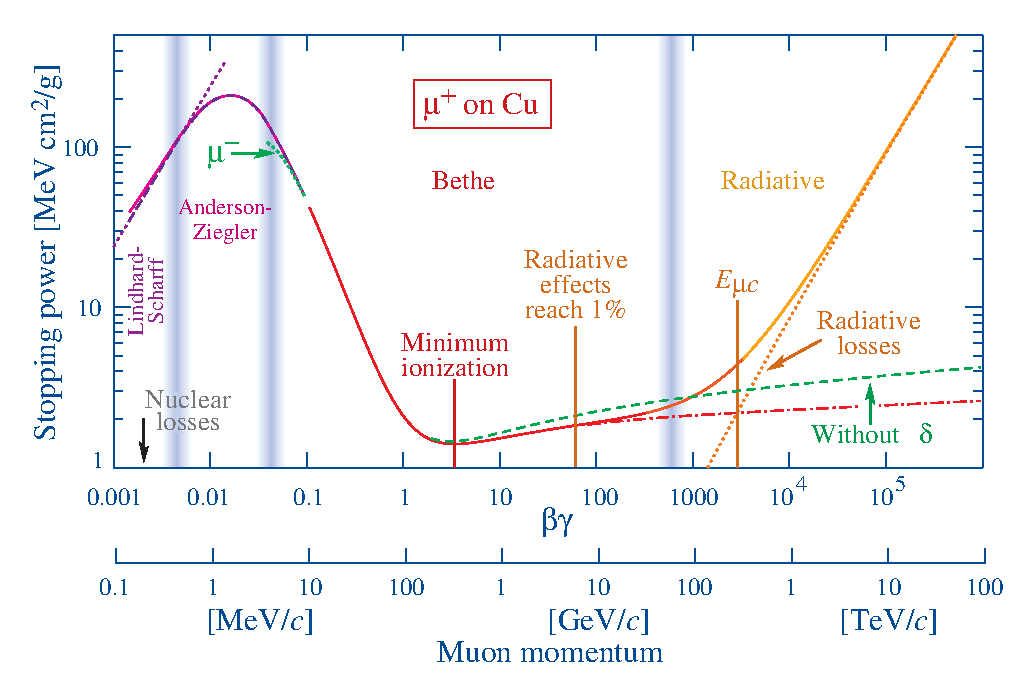
\includegraphics{plots/Chap2/rpp_icru49_cu_col.eps}
      }
    \end{center}
        \caption[Stopping power for positive muons in copper.]
        {\small Stopping power ($\frac{-dE}{dx}$) for positive muons in copper as a function of $\beta\gamma=\frac{p}{Mc}$, see ref.~\cite{PDG}.} 
            \label{StoppingMuon}
\end{figure}

It is now worth noticing that the dominant interaction mechanism for high energy photons is pair production, which results in a high energy electron/positron pair, and that high energy charged particles lose energy primarily by emitting photons.  
With this in mind it's easy to imagine that a single high energy EM particle will lead to a large cascade of lower energy EM particles while travelling through a material.  
These cascading events (known as electromagnetic showers) tend to remain in a narrow cone around the trajectory of the instigating particle, with the tightness of the cone being independent of the initial energy of the particle (see Moli{\`e}re radius in~\cite{grupen_shwartz_2011}).  
Another feature of electromagnetic showers is that, relatively speaking, they do not penetrate very deeply into the material.   
These are some variables that will be useful in identifying EM showers, with how they identified within ATLAS being briefly discussed in Sec.~\ref{EMReco}. 

\begin{table}
  \centering
  \begin{tabular}{ |c|c|c|}
  \hline
  \multicolumn{3}{|c|}{\textbf{EM calorimeter}} \\
  \hline
  \hline
  \multicolumn{3}{|c|}{Longitudinal layers, $\eta$ coverage} \\
  \hline
  Presampler  & 1, $\mid\eta\mid<1.52$            & 1, $1.5<\mid\eta\mid<1.8$ \\
  \hline
  Calorimeter & 3, $\mid\eta\mid<1.35$            & 2, $.1375<\mid\eta\mid1.5$ \\
              & 2, $1.35<\mid\eta\mid<1.475$      & 3, $1.5<\mid\eta\mid<2.5$ \\
              &                                   & 2, $2.5<\mid\eta\mid<3.2$ \\
  \hline
  FCal        &                                   & 1, $3.1<\mid\eta\mid < 4.9$ \\
  \hline
  \multicolumn{3}{|c|}{Granularity $\Delta\eta x \Delta\phi$} \\
  \hline
  Presampler  & 0.025 x 0.1, $\mid\eta\mid<1.52$                & 0.025 x 0.1, $1.5<\mid\eta\mid<1.8$ \\
  \hline
  Calorimeter layer 1 & 0.003 x 0.1, $\mid\eta\mid<1.4$         & 0.05 x 0.1,  $1.375<\mid\eta\mid<1.425$ \\
                      & 0.025 x 0.025, $1.4<\mid\eta\mid<1.475$ & 0.025 x 0.1, $1.425<\mid\eta\mid<1.5$ \\
                      &                                         & 0.003 x 0.1, $1.5<\mid\eta\mid<1.8$ \\
                      &                                         & 0.004 x 0.1, $1.8<\mid\eta\mid<2.0$ \\
                      &                                         & 0.006 x 0.1, $2.0<\mid\eta\mid<2.4$ \\
                      &                                         & 0.025 x 0.1, $2.4<\mid\eta\mid<2.5$ \\
                      &                                         & 0.1 x 0.1,   $2.5<\mid\eta\mid<3.2$ \\
  \hline
  Calorimeter layer 2 & 0.025 x 0.025, $\mid\eta\mid<1.4$       & 0.05 x 0.025,$1.375<\mid\eta\mid<1.425$ \\
                      & 0.075 x 0.025, $1.4<\mid\eta\mid<1.475$ & 0.025 x 0.025, $1.425<\mid\eta\mid<2.5$ \\
                      &                                         & 0.1 x 0.1, $2.5<\mid\eta\mid<3.2$ \\
  \hline
  Calorimeter layer 3 & 0.05 x 0.025, $\mid\eta\mid<1.35$       & 0.05 x 0.025, $1.5<\mid\eta\mid<2.5$ \\
  \hline
  FCal                &                                         & 0.2 x 0.2, $3.1<\mid\eta\mid < 4.9$ \\
  \hline
  \end{tabular}
  \caption[Main parameters of the electromagnetic calorimeter system. ]
        {\small Main parameters of the electromagnetic calorimeter system in ATLAS~\cite{JOIATLAS} }
\label{table:EMCalo}
\end{table}

The ATLAS detector makes use of what are known as sampling calorimeters.  
A sampling calorimeter is a calorimeter which alternates back and forth between a dense material which is used to advance the particle shower (absorbers) and an active material which measures the shower deposits.  
While there is a disadvantage to this design with energy deposited in the absorber being invisible to the detector, having the full energy of the particle being deposited in a shorter length of material allows for a reduction in size of any additional detectors beyond the calorimeter.  
In both the barrel and endcaps the absorber for the EM calorimeter is lead and the active material is liquid argon (LAr), while in the forward region a copper/LAr detector is used.  
When charged particles pass through the active medium the liquid argon is ionized and the charge is collected on kapton electrodes, which is how the energy measurement is made.  
A breakdown of how the number of sampling layers and the resolution of the EM calorimeter vary with $\eta$ in the central and endcap regions can be seen in Table~\ref{table:EMCalo}.  


\subsubsection{Hadronic Calorimeter}
\label{Had}
It is very easy to see many similarities between EM calorimeters and hadronic calorimeters.  
Hadronic calorimeters rely on both electromagnetic and strong interactions between the particles to be measured and the detector, where these interactions produce secondary particles.  
This process, known as a hadronic shower, continues until the secondary particles reach a low enough energy that they are fully absorbed by the material and their energy measured.  
The differences between hadronic and electromagnetic showers tend to be in the size, both in depth and width, of the showers (with hadronic showers being larger in both dimensions) and the event by event variations of the showers (with hadronic showers being subject to much larger fluctuations).  

As the lowest mass hadron is over 200 times more massive than the electrons ($\pi^{0}$ at 145 MeV) it is save to assume that at energies which will be achieved in the ATLAS detector bremsstrahlung will not be an important energy loss mechanism for hadrons.  
Ionization and excitation on the other hand are still relevant contributors to the overall energy loss of hadrons.  
The rate at which energy is lost via these mechanisms for particles which are heavier than an electron is described by the Bethe-Bloch formula,  
\begin{equation}
-\frac{\mathrm{d}E}{\mathrm{d}x}=\frac{2CZz^2}{A\beta^2}\left[\mathrm{ln}\left(a\gamma^2\beta^2\right)-\beta^2-\frac{\delta}{2}\right], 
\end{equation}
where $C$ is some constant, $z$ is the charge of the particle in question, $Z$ and $A$ are the atomic number and weight of the material being ionized, $\beta$ and $\gamma$ are the velocity and Lorentz factor of the incident particle, $\delta$ is a parameter describing density effects, and $a$ depends on the electron mass and ionization energy of the absorber.  

While these particles do interact electromagnetically it is the interactions between the hadrons and the atomic nuclei via the strong force (resulting in secondary hadrons) which account for the majority of the energy loss.  
The average distance between these interactions is much larger than the radiation length which is the cause of the extra penetration depth of these showers when compared to their EM counterparts.  
To get an idea of the difference in penetration depth between hadronic and electromagnetic showers one needs only to pick a material, say copper, and compare the average distance between hadronic interactions $\lambda_{\mathrm{int}}$ (15 cm in copper) to the radiation length $\chi_{0}$ in the same material (1.4 cm)~\cite{Wigmans2008}.  
The large width of hadronic showers is caused by large transverse momentum transfers in these nuclear interactions.  

\begin{table}
  \centering
  \begin{tabular}{ |c|c|c|}
  \hline
  \multicolumn{3}{|c|}{\textbf{Hadronic calorimeter}} \\
  \hline
  \hline
  \multicolumn{3}{|c|}{Tile calorimeter} \\
  \hline 
                     & Barrel                                   & Extended barrel \\
  Coverage           & $\mid\eta\mid<1.0$                       & $0.8<\mid\eta\mid<1.7$ \\
  \hline 
  Number of layers   & 3                                        & 3 \\
  \hline 
  Granularity        & 0.1 x 0.1				& 0.1 x 0.1 \\
  Last layer only    & 0.2 x 0.1				& 0.2 x 0.1 \\
  \hline 
  \hline
  \multicolumn{3}{|c|}{Hadronic endcaps} \\
  \hline 
  Coverage           & 	\multicolumn{2}{|c|}{$1.5<\mid\eta\mid<3.2$} \\
  \hline
  Number of layers   &  \multicolumn{2}{|c|}{ 4} \\
  \hline
  Granularity        & 	\multicolumn{2}{|c|}{0.1 x 0.1, $1.5<\mid\eta\mid<2.5$} \\
  		     &  \multicolumn{2}{|c|}{ 0.2 x 0.2, $2.5<\mid\eta\mid<3.2$} \\
  \hline
  \hline
  \multicolumn{3}{|c|}{Forward calorimeter} \\
  \hline
  Coverage	     & \multicolumn{2}{|c|}{$3.1<\mid\eta\mid<4.9$} \\
  \hline
  Number of layers   & \multicolumn{2}{|c|}{2} \\
  \hline
  Granularity        & \multicolumn{2}{|c|}{$\approx$ 0.2 x 0.2} \\
  \hline
  \end{tabular}
  \caption[Main parameters of the hadronic calorimeter system. ]
        {\small Main parameters of the hadronic calorimeter system in ATLAS~\cite{JOIATLAS}. }
%1748-0221-3-08-S08003} }
\label{table:HadCalo}
\end{table}

While a large number of the particles resulting from the nuclear interactions will be pions ($\approx$ 90 \%), other particles like protons, neutrons, kaons, etc. are also produced.  
On average the three pion flavours ($\pi^0$, $\pi^{+}$, and $\pi^{-}$) are produced in with equal frequency, with large variations in make up of the secondaries being possible between any two given interactions.  
Interestingly charged pions interact with matter much differently than their neutral counterparts.  
Where charged pions have a mean lifetime $\tau$ of 2.6 x $10^{-8}$ s ($\tau c$ = 7.8 m) and will tend to have a further nuclear interactions before decaying, neutral pions have a much shorter lifetime ($\tau c$ = 25 nm) leading them to quickly decay into a pair of photons which will initiate EM showers within the hadronic shower~\cite{PDG}.  
As a result of this important difference the amount of detectable energy deposited in a calorimeter from a hadronic shower can have a strong dependence on what fraction of pions from the first few interactions happen to have been neutral.  

The fraction of the total energy deposited in the calorimeter by these small EM sub showers ($f_{em}$) varies as a function of the energy of the particle initiating the shower, increasing from $\approx$ 30\% for particles at 10 GeV to $\approx$ 50\% for particles at 100 GeV.  
The rest of the energy can be accounted for as follows: 34\% is used to overcome the atomic binding potential to release protons and neutrons (so called invisible energy), 10\% is in low energy (typically 3 MeV) neutrons which have been released from nuclei, and 56\% is deposited via ionizing particles, where 2/3 of that is via protons~\cite{Wigmans2008}.  
This is all to say that a large portion of the non-EM energy is deposited in the calorimeter via low energy free nucleons and not relativistic pions.  

The hadronic calorimeter, just like the EM calorimeter, is a sampling calorimeter.  
The similarities go even further in that in both the FCal and endcaps the active material for the hadronic calorimeter is LAr, with the absorber in the endcaps being copper and the absorber in the forward region being tungsten.  
In the barrel the hadronic calorimeter uses steel as the absorber material and a plastic scintillator as the active material.  
The number of sampling layers and the granularity of each of these regions of the hadronic calorimeter can be seen in Table.~\ref{table:HadCalo}. 

\subsection{ATLAS Hardware: Muon Spectrometer}
Muons are 200 times heavier than electrons, and are therefore typically minimum ionizing at the LHC and therefore do not produce electromagnetic showers.  
Since muons also do not carry any colour charge they do not produce hadronic showers either.  
Thankfully as they are charge carriers they do interact with the tracking systems in the inner detector, and with the help of a second tracking system beyond the hadronic calorimeter they become easy to identify as they are the only ionizing particle which will regularly pass through the entire calorimeter.  
The magnetic field for the muon spectrometer is provided large superconducting air-core toroids, with the field in the central region ($\mid\eta\mid<$ 1.4) being provided by the barrel toroid and in the forward regions (1.6 $<\mid\eta\mid<$ 2.7) is is provided by two smaller endcap magnets.  
In the transition regions the magnetic fields are provided by a combination of these three magnets.  

In the central barrel region the muon hits are measured in three separate layers (stations) which arranged in concentric cylinders with radii of about 5, 7.5, and 10 m~\cite{MuonTDR}.  
These distances are chosen to measure the muons position as they enter, are at the midpoint, and again as they exit the magnetic field to best measure the change in the momentum of the muons.  
The two endcaps are made up of four wheels at distances of 7.4, 10.8, 14, and 21.5 m, where the additional wheel at 10.8 m is allow for the full three measurements of the muons trajectory in the region which is uncovered by the outermost wheel (see Fig.~\ref{MuonSpectroFig}).  

\begin{figure}[!ht]
  \begin{center}
    \scalebox{0.5}{        
      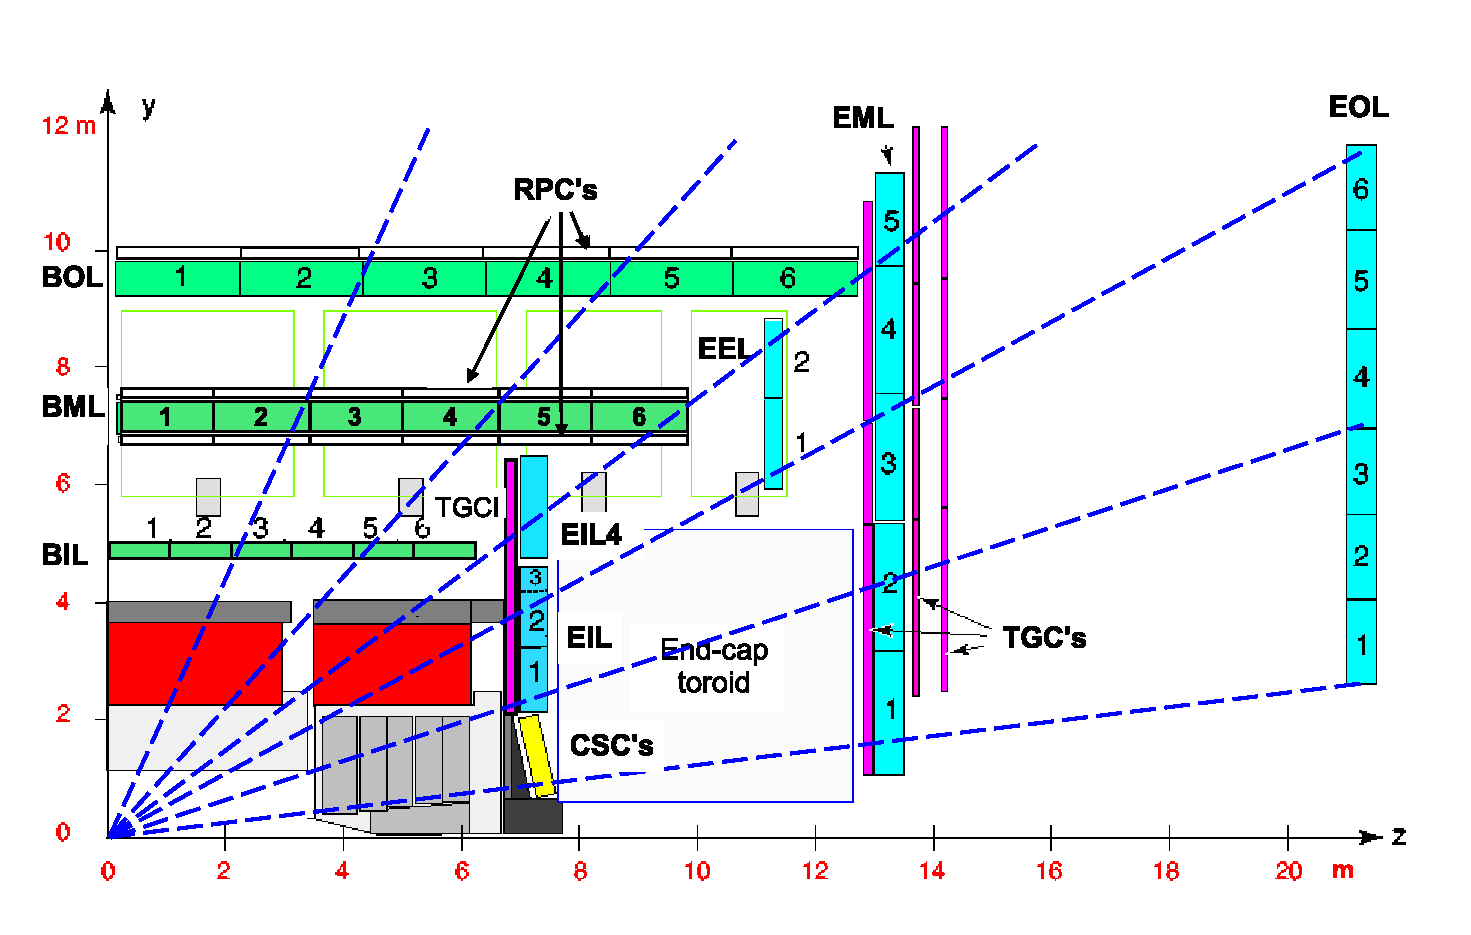
\includegraphics{plots/Chap2/Muon_rz_large_sect_6.eps}
    }
  \end{center}
  \caption[Stopping power for positive muons in copper.]
      {\small Cross-section of the muon system in a plane containing the beam axis (bending plane). Infinite-momentum muons would propagate along straight trajectories which are illustrated by the dashed lines and typically traverse three muon stations~\cite{JOIATLAS}.}
  \label{MuonSpectroFig}
\end{figure}

Monitored Drift Tubes (MDT's) are used to make these position measurements in the outer two layers of the muon spectrometer over the full eta range ($\mid\eta\mid<$ 2.7), and they are also used in all but the most forward portion of the inner most layer as well ($\mid\eta\mid<$ 2.0).  
MDT's make use of the trail of ionized particles left behind as a charged particle passes through a material in the same way as the TRT (see Sec.~\ref{Sec.ID}).  
 
 

\subsection{Triggers}
\label{Trig}
During both 2015 and 2016 the LHC has been bringing two bunches of protons to collide at the centre of the ATLAS detector every 25 ns.  
With each even potentially taking up to 2 MB to store both recording and storing all of this data can be a problem.  
To further extend the problem the large majority of these collision events will be elastic collisions or low Pt dijet events which are of little interest in this high energy environment.  
The solution to this problem is to only record a certain fraction of the total number of events that have been provided.  
This must be done in a way which maximizes the number of rare events recorded while simultaneously removing as many low interest events as possible.  
The triggering system uses a combination of hardware and software decision makers to perform exactly this task~\cite{Run2Triggers}.  

The trigger system is broken down into two parts with the first part being the L1 trigger.  
The L1 trigger is hardware based and reduces the number of events to be considered from 40 MHz per second down to 100 kHz.  
It uses a more course object definition than the full reconstruction, but selections can still be made based on energy thresholds for given objects, as well as more topological information like isolation requirements or a specified range for the invariant mass of a combination of objects.  

The second stage of the trigger system is known as the higher level trigger, or HLT.  
In the HLT some full offline like unseeded reconstruction algorithms can be run, including topoclustering and muon reconstruction.  
This is not always the case, for example time considerations necessitate the use of an offline like track reconstruction algorithm that makes use of some L1 tracking information.  
The HLT is designed to reduce the event rate from the 100 kHz output of the L1 trigger down to 600 Hz, which can be increased to 1-1.5 kHz at peak luminosities.  

While these triggers can be very efficient at selection relatively rare more `interesting' events to be recorded for future study, not all event topologies desired by the various physics groups in the ATLAS collaboration are infrequent enough that every instance of that event can be stored.  
The compromise that's made for these high rate events is that for a given trigger an additional requirement is added to the trigger which is satisfied randomly with only a preset probability of passing (prescaling).  
The true number of events of these types which have actually occurred can then be approximated using that random acceptance rate.  
 
 
 





